% This LaTeX was auto-generated from MATLAB code.
% To make changes, update the MATLAB code and export to LaTeX again.

\documentclass{article}

\usepackage[utf8]{inputenc}
\usepackage[T1]{fontenc}
\usepackage{lmodern}
\usepackage{graphicx}
\usepackage{color}
\usepackage{hyperref}
\usepackage{amsmath}
\usepackage{amsfonts}
\usepackage{epstopdf}
\usepackage[table]{xcolor}
\usepackage{matlab}

\sloppy
\epstopdfsetup{outdir=./}
\graphicspath{ {./Lab04_images/} }

\begin{document}

\matlabtitle{LAB 4: SIMULATION OF ANGULAR VELOCITY CONTROL FOR A DC MOTOR}

\begin{matlabcode}
%---------------------------------------
% Fill in your student Name and ID.
Students.Name = 'Seyed Yazdan Zinati';
Students.ID = '260928077';
%---------------------------------------
\end{matlabcode}


\matlabheading{\textbf{0. Objectives}}

\begin{par}
\begin{flushleft}
In this lab, we will run different simulation experiments to track a desired reference signal with a simulated DC Motor. We will first run an open-loop experiment, then we will use state feedback to control the angular velocity of DC motor.
\end{flushleft}
\end{par}

\matlabheading{\textbf{1. A State-Space Representation of DC Motor}}

\begin{par}
\begin{flushleft}
A DC motor is a device that converts armature current into mechanical torque. A schematic of a DC motor is shown in the following
\end{flushleft}
\end{par}

\begin{par}
\begin{flushleft}
\textless{}\textless{}fig\_dcmotorshematic.png\textgreater{}\textgreater{}
\end{flushleft}
\end{par}

\begin{par}
\begin{flushleft}
We can model the DC motor using the armature current $i$ and the angular speed $\omega$. The dynamics of the DC motor are given by the following two coupled differential equations:
\end{flushleft}
\end{par}

\begin{par}
$$J{{\frac{d\omega }{dt}+b\omega =K_t i}}$$
\end{par}

\begin{par}
$$L{{\frac{di}{dt}+Ri=v-K_e \omega }}$$
\end{par}

\begin{par}
\begin{flushleft}
where the parameters are defined as follow
\end{flushleft}
\end{par}

\begin{matlabcode}
Param.Kt = 0.034; % Torque proportionality constant (Kg m2 /s2/A) (N.m/A)
Param.Ke = 0.034; % Back electromotive proportionality constant (V/rad/s)
Param.L = 0.018; % Electric inductance (H)
Param.R = 8.4; % Terminal resistance (Ohm)
Param.J = 2e-05; % Rotor moment of inertia (kg.m2)
Param.b = 1e-06; % Rotor viscous friction constant (Kg.m2/s) (N.m.s)
\end{matlabcode}


\begin{par}
\begin{flushleft}
From these differential equations we can represent the DC Motor model by the following state-space representation
\end{flushleft}
\end{par}

\begin{par}
$${{\frac{d}{dt}x(t)=\left(\begin{array}{cc}
-{{\frac{b}{J}}} & {{\frac{K_t }{J}}}\\
-{{\frac{K_e }{L}}} & -{{\frac{R}{L}}}
\end{array}\right)x(t)+\left(\begin{array}{c}
0\\
{{\frac{1}{L}}}
\end{array}\right)v(t)}}$$
\end{par}

\begin{par}
\begin{flushleft}
where $v(t)$ is the voltage and the state vector contains the angular velocity $\omega (t)$ and the current $i(t)$
\end{flushleft}
\end{par}

\begin{par}
$$x(t)=\left(\begin{array}{c}
\omega (t)\\
i(t)
\end{array}\right)$$
\end{par}

\matlabheading{\textit{Question 1 (1 mark)}}

\begin{par}
\begin{flushleft}
Write the state-space representation of the DC Motor (Only A and B matrices).
\end{flushleft}
\end{par}

\begin{matlabcode}
A = [-Param.b/Param.J, Param.Kt/Param.J; -Param.Ke/Param.L, -Param.R/Param.L]
\end{matlabcode}
\begin{matlaboutput}
A = 2x2    
1.0e+03 *

   -0.0000    1.7000
   -0.0019   -0.4667

\end{matlaboutput}
\begin{matlabcode}
B = [0; 1/Param.L]
\end{matlabcode}
\begin{matlaboutput}
B = 2x1    
         0
   55.5556

\end{matlaboutput}


\matlabheading{\textbf{2. Desired specifications}}

\begin{par}
\begin{flushleft}
The objective of this lab is to track a reference signal $\omega_{ref}$ while satisfying the following requirements:
\end{flushleft}
\end{par}

\begin{itemize}
\setlength{\itemsep}{-1ex}
   \item{\begin{flushleft} Overshoot less than 10\%. \end{flushleft}}
   \item{\begin{flushleft} 5\%-settling time less than 0.2 seconds. \end{flushleft}}
   \item{\begin{flushleft} Steady state gain of 1 $\pm$ 5\%. \end{flushleft}}
\end{itemize}

\begin{par}
\begin{flushleft}
The Reference angular velocity is defined by the following:
\end{flushleft}
\end{par}

\begin{par}
$$\omega_{ref} (t)=\left\lbrace \begin{array}{cc}
0, & 0\le t<1\\
50, & t\ge 1
\end{array}\right.$$
\end{par}

\begin{par}
\begin{flushleft}
In \texttt{\textbf{MATLAB}} we define $\omega_{ref}$ by:
\end{flushleft}
\end{par}

\begin{matlabcode}
T = 10; % Simulation duration
dt = 0.01; % Simulation step time
t = (0:dt:T)'; % Time array
TStart = 1; % Step start
wRef = zeros(size(t));
wRef(t >= TStart) = 50; % rad/s

figure;
clf;
plot(t, wRef, 'LineWidth', 2.0)
legend('Reference angular velocity (rad/s)');
xlim([0, T])
ylim([0, 80])
title(sprintf('Student ID %s - Reference angular velocity', Students.ID));
grid on
\end{matlabcode}
\begin{center}
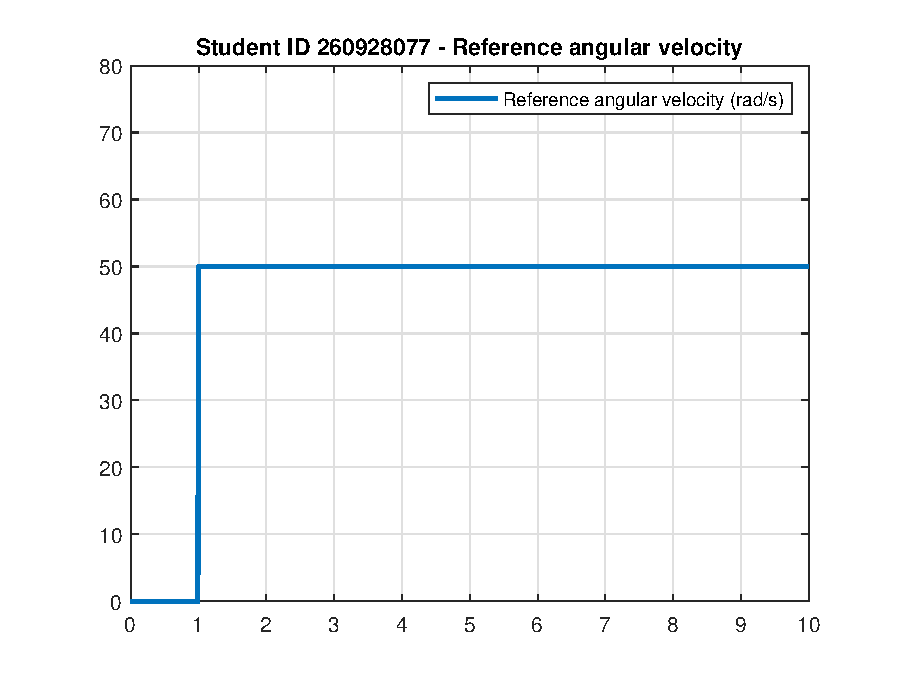
\includegraphics[width=\maxwidth{56.196688409433015em}]{figure_0.eps}
\end{center}


\matlabheading{\textbf{3. Open-loop Simulation Experiment}}

\begin{par}
\begin{flushleft}
The state-space open-loop system is presented below.
\end{flushleft}
\end{par}

\begin{par}
\begin{flushleft}
\textless{}\textless{}fig\_lab04\_openloopdiagram.png\textgreater{}\textgreater{}
\end{flushleft}
\end{par}

\begin{par}
\begin{flushleft}
Note that if we think of the angular velocity $\omega (t)$ as the output of this system, then $C=\left(\begin{array}{cc}
1 & 0
\end{array}\right)$ and
\end{flushleft}
\end{par}

\begin{par}
$$\omega (t)=Cx(t)$$
\end{par}

\begin{par}
\begin{flushleft}
In this case, the transfer function from the voltage $v(t)$ to the angular velocity $\omega (t)$ is given by
\end{flushleft}
\end{par}

\begin{par}
$$G_o (s)=C(sI-A)^{-1} B$$
\end{par}

\begin{par}
\begin{flushleft}
In \texttt{\textbf{MATLAB}}, we can find the transfer function of a state-space model using the function \texttt{\textbf{ss}} and \texttt{\textbf{tf}}, as shown below.
\end{flushleft}
\end{par}

\begin{matlabcode}
C = [1, 0];
D = 0;
Go = ss(A, B, C, D)
\end{matlabcode}
\begin{matlaboutput}
Go =
 
  A = 
           x1      x2
   x1   -0.05    1700
   x2  -1.889  -466.7
 
  B = 
          u1
   x1      0
   x2  55.56
 
  C = 
       x1  x2
   y1   1   0
 
  D = 
       u1
   y1   0
 
Continuous-time state-space model.
\end{matlaboutput}
\begin{matlabcode}
tf(Go)
\end{matlabcode}
\begin{matlaboutput}
ans =
 
        9.444e04
  --------------------
  s^2 + 466.7 s + 3234
 
Continuous-time transfer function.
\end{matlaboutput}


\matlabheading{\textit{Question 2 (1 mark)}}

\begin{par}
\begin{flushleft}
Recall that the DC gain can be obtained from a Laplace transfer function, by setting the laplace variable $s$ to zero. From the state-space model representation $(A,\,B,\,C,\,D)$, calculate the DC gain.
\end{flushleft}
\end{par}

\begin{matlabcode}
% dcGainOL = 9.444e04/3234
dcGainOL = dcgain(Go)
\end{matlabcode}
\begin{matlaboutput}
dcGainOL = 29.1996
\end{matlaboutput}


\begin{par}
\begin{flushleft}
Observe that if the open-loop system is a stable system. The DC Motor will be responded to a reference step signal without using a controller. However, the response will be determined by the eigenvalues of the open-loop $A$ matrix (or equivalently, the poles of the open-loop transfer function).
\end{flushleft}
\end{par}

\matlabheading{\textit{Question 3 (1 mark)}}

\begin{par}
\begin{flushleft}
Determine the poles of the open-loop transfer function from the state-space matrix $A$ (Hint: \texttt{\textbf{help eig}}). Is the system stable? (Justify your answer.)
\end{flushleft}
\end{par}

\begin{matlabcode}
eigenvalues = eig(A);

p1 = eigenvalues(1)
\end{matlabcode}
\begin{matlaboutput}
p1 = -7.0363
\end{matlaboutput}
\begin{matlabcode}
p2 = eigenvalues(2)
\end{matlabcode}
\begin{matlaboutput}
p2 = -459.6804
\end{matlaboutput}


\begin{matlabcode}
% We can observe that the eigenvalues of A (or equivalently the poles of
% the open-loop transfer funtion) are both negative and therefore situated
% in the LHP. So the system is stable.
\end{matlabcode}


\begin{par}
\begin{flushleft}
Following a fixed input $v_0$ the angular velocity $\omega$ will attain a steady angular velocity $\omega_{\infty } =DC_{gain} v_0$.
\end{flushleft}
\end{par}

\begin{par}
\begin{flushleft}
We can simulate the response of an LTI system to an arbitrary input using the \texttt{\textbf{lsim}} function.
\end{flushleft}
\end{par}

\matlabheading{\textit{Question 4 (0.5 mark)}}

\begin{par}
\begin{flushleft}
Complete the following code to simulate the response of the system to a 1 volt input signal, and plot the results.
\end{flushleft}
\end{par}

\begin{matlabcode}
v = ones(size(t)); % create a signal with one volt.
w = lsim(Go, v, t);

% Plot results
figure;
clf;

% plot the angular velocity w
plot(t, w)

legend('Angular velocity (rad/s)', ...
    'location', 'best');
xlim([0, T])
ylim([0, 40])
title(sprintf('Student ID %s - Simulation of 1 volt step', Students.ID));
grid on
\end{matlabcode}
\begin{center}
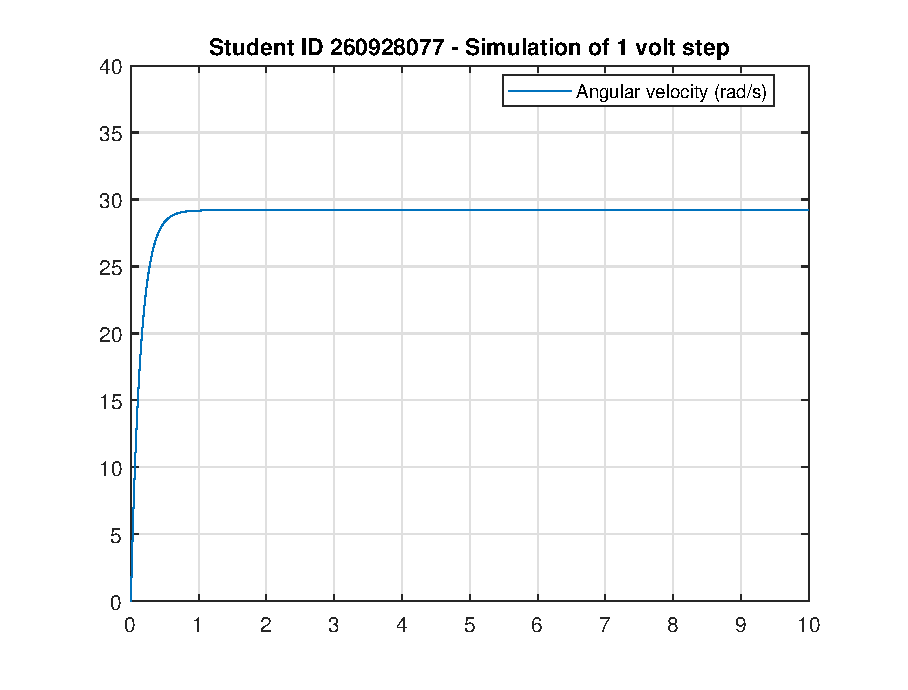
\includegraphics[width=\maxwidth{56.196688409433015em}]{figure_1.eps}
\end{center}


\begin{par}
\begin{flushleft}
In open-loop we can generate the voltage $v$ from $\omega_{ref}$ through the gain $N_o$.
\end{flushleft}
\end{par}

\begin{par}
$$v(t)=N_o \omega_{ref} (t)$$
\end{par}

\matlabheading{\textit{Question 5 (1 mark)}}

\begin{par}
\begin{flushleft}
Find the value of $N_o$ such the final value of the angular velocity output $\omega$ is the same as $\omega_{ref}$ (i.e. 50 rad/s)
\end{flushleft}
\end{par}

\begin{matlabcode}
% No = 0.03425 (Found using an experimental method) 

No = 1/dcGainOL
\end{matlabcode}
\begin{matlaboutput}
No = 0.0342
\end{matlaboutput}
\begin{matlabcode}

% The voltage is generated from wRef and No
v = No * wRef;
% Simulate the output angular velocity using lsim
w = lsim(Go, v, t);


% Plot results
figure;
clf;
hold on
% Superpose the angular velocity w and the reference wRef
plot(t, w)
plot(t, wRef, 'r')

legend('Angular velocity (rad/s)', ...
    'Reference angular velocity (rad/s)', ...
    'location', 'best');
xlim([0, T])
ylim([0, 80])
title(sprintf('Student ID %s - Open-loop tracking Simulation', Students.ID));
grid on
\end{matlabcode}
\begin{center}
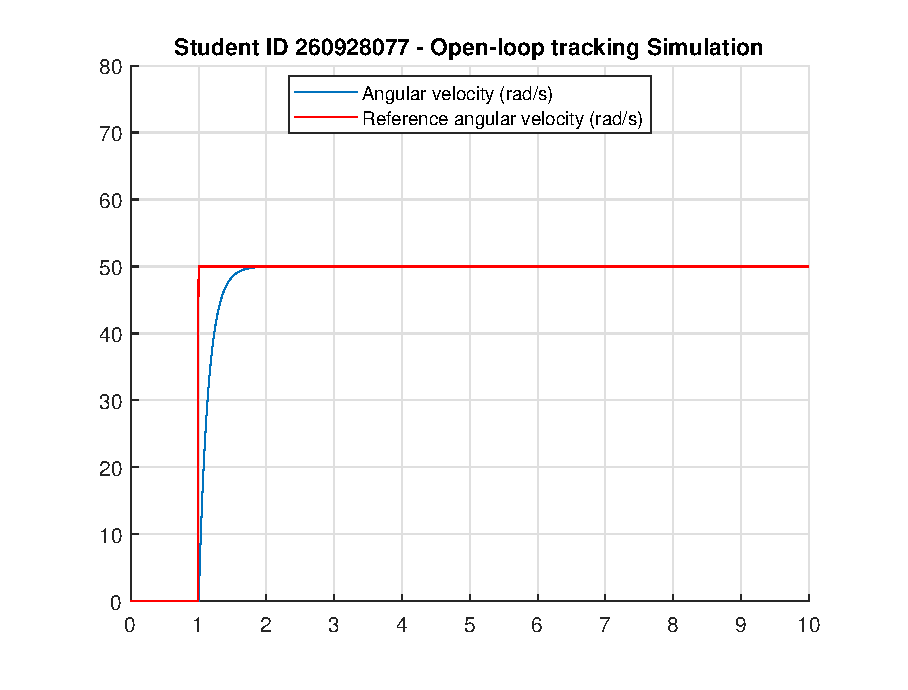
\includegraphics[width=\maxwidth{56.196688409433015em}]{figure_2.eps}
\end{center}
\begin{matlabcode}


\end{matlabcode}


\matlabheading{\textit{Question 6 (0.5 marks)}}

\begin{par}
\begin{flushleft}
Based on the plot above, determine if all the requirements are satisfied. Justify your answer.
\end{flushleft}
\end{par}


\vspace{1em}
\begin{matlabcode}
stepinfo(w, "SettlingTimeThreshold", 0.05)
\end{matlabcode}
\begin{matlaboutput}
ans = 
        RiseTime: 31.2225
    SettlingTime: 143.8004
     SettlingMin: 45.0198
     SettlingMax: 50.0000
       Overshoot: 0
      Undershoot: 0
            Peak: 50.0000
        PeakTime: 593

\end{matlaboutput}
\begin{matlabcode}
finalW = mean(w(t>=6));
finalWred = mean(wRef(t>=6));
SSgain = finalW/finalWred
\end{matlabcode}
\begin{matlaboutput}
SSgain = 1.0000
\end{matlaboutput}
\begin{matlabcode}

% We had the following requirements defined in 2. : 
% 1 - Overshoot less than 10%
% 2 - 5%-settling time less than 0.2 seconds
% 3 - Steady state gain of 1±5%

% We can see from the above plot that the OS% is 0 so OS% requirements are
% met. The 5% settling time is about 0.438 s which is larger than the 0.2 s
% to satisfy our requirements. So the settling time doesn't meet our
% requirements. The SS gain is also very close to 1 and withing our defined
% error bound of 5%. 

% So as the requirements for Ts are not met, not all 
% the requirements are satisfied based on the above plot. 
\end{matlabcode}

\begin{par}
\begin{flushleft}
 
\end{flushleft}
\end{par}

\matlabheading{\textbf{4. Closed-Loop Simulation Experiment}}

\begin{par}
\begin{flushleft}
The closed-loop system is presented in the following figure.
\end{flushleft}
\end{par}

\begin{par}
\begin{flushleft}
\textless{}\textless{}fig\_lab04\_clsoedloopdiagram1.png\textgreater{}\textgreater{}
\end{flushleft}
\end{par}

\begin{par}
\begin{flushleft}
The full-state feedback control law is defined as follow
\end{flushleft}
\end{par}

\begin{par}
$$v(t)=N_c \omega_{ref} -Kx(t)$$
\end{par}

\begin{par}
\begin{flushleft}
where gain $K$ is a 1 by 2 matrix and the gain $N_c$ is forward gain that will ensure achieving $\omega_{ref}$ at steady state.
\end{flushleft}
\end{par}

\begin{par}
\begin{flushleft}
Actually, this diagram is equivalent to an open-loop diagram but with a different state transition matrix $A_{cl} =A-BK$
\end{flushleft}
\end{par}

\begin{par}
\begin{flushleft}
\textless{}\textless{}fig\_lab04\_clsoedloopdiagram2.png\textgreater{}\textgreater{}
\end{flushleft}
\end{par}

\begin{par}
\begin{flushleft}
Doing a state feedback with gain $K$ is equivalent to changing the system dynamics from $A$ to $A-BK$. Recall that the eigenvalues of a state transition matrix $A$ are the poles of the system.
\end{flushleft}
\end{par}

\begin{par}
\begin{flushleft}
We want to choose $K$ to specify the new poles of the closed-loop system $A-BK$ in a way that satisfies the desired specifications
\end{flushleft}
\end{par}

\begin{itemize}
\setlength{\itemsep}{-1ex}
   \item{\begin{flushleft} Overshoot less than 10\%. \end{flushleft}}
   \item{\begin{flushleft} 5\%-settling time less than 0.2 seconds. \end{flushleft}}
\end{itemize}

\begin{par}
\begin{flushleft}
Then we will choose $N_c$ similarly to the open-loop section to satisfy the steady state requirements:
\end{flushleft}
\end{par}

\begin{itemize}
\setlength{\itemsep}{-1ex}
   \item{\begin{flushleft} Steady state gain of 1 $\pm$ 5\%. \end{flushleft}}
\end{itemize}

\matlabheading{\textit{Question 7 (2 marks)}}

\begin{par}
\begin{flushleft}
Calculate the desired poles that satisfies the specifications (Use formula sheet for transient response of 2nd order system in myCourses if needed):
\end{flushleft}
\end{par}

\begin{par}
\begin{flushleft}
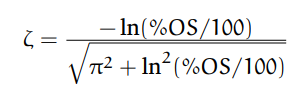
\includegraphics[width=\maxwidth{30.005017561465127em}]{image_0} 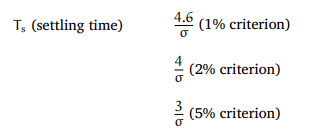
\includegraphics[width=\maxwidth{31.510286001003514em}]{image_1}
\end{flushleft}
\end{par}

\begin{matlabcode}
% we use the 2 above expressions to find zeta and wn to subsitute in
% Poles = -zeta*wn (+/-) wn*sqrt(zeta^2 - 1)


zeta = -(log(10/100))/sqrt(pi.^2 + (log(10/100)).^2)
\end{matlabcode}
\begin{matlaboutput}
zeta = 0.5912
\end{matlaboutput}
\begin{matlabcode}

% 3/(wn*zeta) = 0.2
wn = 3/(zeta*0.2)
\end{matlabcode}
\begin{matlaboutput}
wn = 25.3741
\end{matlaboutput}
\begin{matlabcode}


p1d = -zeta*wn + wn * sqrt(zeta^2 - 1)
\end{matlabcode}
\begin{matlaboutput}
p1d = -15.0000 + 20.4656i
\end{matlaboutput}
\begin{matlabcode}
p2d = -zeta*wn - wn * sqrt(zeta^2 - 1)
\end{matlabcode}
\begin{matlaboutput}
p2d = -15.0000 - 20.4656i
\end{matlaboutput}


\begin{par}
\begin{flushleft}
Instead of manual calculation of the value of the gain $K$ that place the poles of $A-BK$ at [p1d, p2d], we will use the \texttt{\textbf{place}} command to calculate the gain $K$
\end{flushleft}
\end{par}

\begin{matlabcode}
K = place(A, B, [p1d, p2d]);
\end{matlabcode}


\matlabheading{\textit{Question 8 (1 mark)}}

\begin{par}
\begin{flushleft}
The closed-loop transfer function is
\end{flushleft}
\end{par}

\begin{par}
$$G_c (s)=C(sI-(A-BK))^{-1} B$$
\end{par}

\begin{enumerate}
\setlength{\itemsep}{-1ex}
   \item{\begin{flushleft} What is the value of the DC gain of the closed-loop system. \end{flushleft}}
   \item{\begin{flushleft} What is the value $N_c$ needed to compensate for the DC gain of the closed-loop system. \end{flushleft}}
\end{enumerate}

\begin{matlabcode}
C = [1, 0];
D = 0;
Gc = ss((A-B*K), B, C, D)
\end{matlabcode}
\begin{matlaboutput}
Gc =
 
  A = 
            x1       x2
   x1    -0.05     1700
   x2  -0.3779   -29.95
 
  B = 
          u1
   x1      0
   x2  55.56
 
  C = 
       x1  x2
   y1   1   0
 
  D = 
       u1
   y1   0
 
Continuous-time state-space model.
\end{matlaboutput}
\begin{matlabcode}
tf(Gc)
\end{matlabcode}
\begin{matlaboutput}
ans =
 
       9.444e04
  ------------------
  s^2 + 30 s + 643.8
 
Continuous-time transfer function.
\end{matlaboutput}
\begin{matlabcode}

% dcGainCL = 9.444e04/643.8
dcGainCL = dcgain(Gc)
\end{matlabcode}
\begin{matlaboutput}
dcGainCL = 146.6887
\end{matlaboutput}


\begin{matlabcode}
Nc = 1/dcGainCL
\end{matlabcode}
\begin{matlaboutput}
Nc = 0.0068
\end{matlaboutput}


\matlabheading{\textit{Question 9 (1 mark)}}

\begin{par}
\begin{flushleft}
Complete the following to simulate angular velocity control with state feedback that tracks the desired $\omega_{ref}$.
\end{flushleft}
\end{par}

\begin{matlabcode}
% Define the closed-loop system using ss : 
% Gc = ss((A-B*K), B, C, D) (Already defined above)


% Simulate the output angular velocity using lsim
w = lsim(Gc, Nc*wRef, t);


% We also simulate the voltage for visualization
v = -lsim(ss(Gc.A, Gc.B, eye(2), Gc.D), Nc*wRef, t) * K' + Nc * wRef;


figure;
clf;
subplot(2, 1, 1)

% Superpose angular velocity w with the angular velocity reference
plot(t, w)
hold on
plot(t, wRef)
hold off

legend('angular velocity (rad/s)', ...
    'Reference angular velocity (rad/s)', ...
    'location', 'best');
xlim([0, T])
ylim([0, 80])
grid on
title(sprintf('Student ID %s - Closed-loop tracking Simulation', Students.ID));

subplot(2, 1, 2)
% Plot the voltage
plot(t, v)

legend('voltage (V)', 'location', 'best');
xlim([0, T])
grid on
\end{matlabcode}
\begin{center}
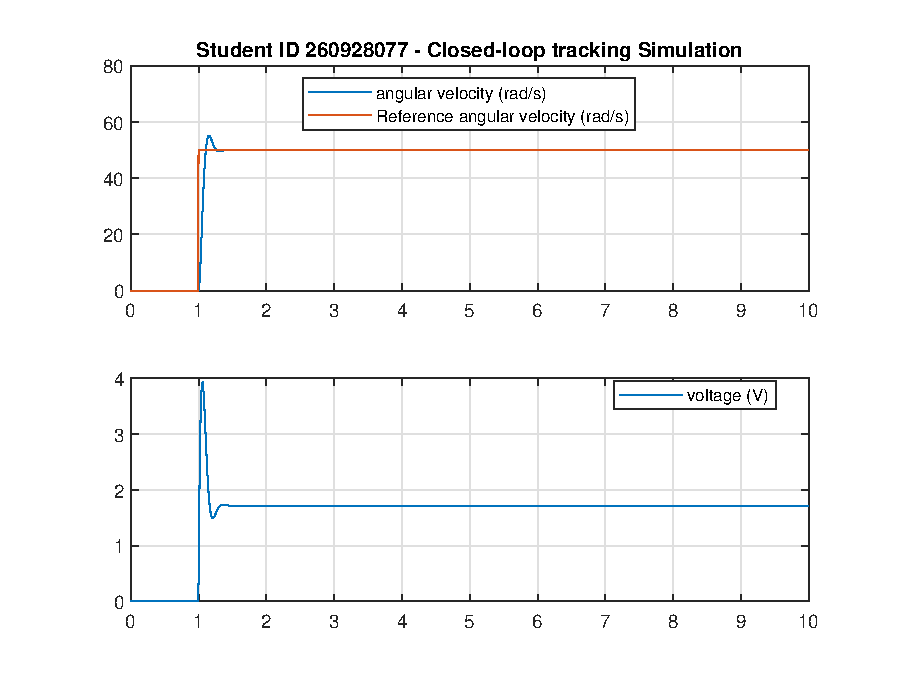
\includegraphics[width=\maxwidth{56.196688409433015em}]{figure_3.eps}
\end{center}


\matlabheading{\textit{Question 10 (1 marks)}}

\begin{par}
\begin{flushleft}
Based on the plot above, determine if all the requirements are satisfied. Justify your answer.
\end{flushleft}
\end{par}

\begin{matlabcode}
stepinfo(w, "SettlingTimeThreshold", 0.05)
\end{matlabcode}
\begin{matlaboutput}
ans = 
        RiseTime: 7.2506
    SettlingTime: 121.6833
     SettlingMin: 47.8410
     SettlingMax: 54.9795
       Overshoot: 9.9590
      Undershoot: 0
            Peak: 54.9795
        PeakTime: 116

\end{matlaboutput}
\begin{matlabcode}
finalW = mean(w(t>=6));
finalWred = mean(wRef(t>=6));
SSgain = finalW/finalWred
\end{matlabcode}
\begin{matlaboutput}
SSgain = 1.0000
\end{matlaboutput}
\begin{matlabcode}


% We had the following requirements defined in 2. : 
% 1 - Overshoot less than 10%
% 2 - 5%-settling time less than 0.2 seconds
% 3 - Steady state gain of 1±5%


% We see an OS% of 9.95 < 10 so OS requirements are met 
% 5% settling time:  0.21 > 0.2 but as we are approxiamting 
% this small error could be tolerated so Ts is satisfied and
% the SS gain is close to 1 and within our 5% error bound.

% So all the requirements are satisfied based on the plot above 
\end{matlabcode}

\end{document}
